\documentclass{article}

\usepackage{lmodern}
\usepackage{hyperref}
\usepackage{amsmath}
\usepackage{mathtools}
\usepackage{amssymb}
\usepackage[T1]{fontenc}
\usepackage{color,graphicx}

\begin{document}

\title{Kernel Based Approaches for Change-Point Detection\\ Multivariate change point analysis}
\date{April 6, 2016}
\author{Anirudhan J. Rajagopalan, ajr619}

\maketitle

\newpage
\section{Change point detection using spectral density}
As per section 4 in~\cite{lavielle2005using}, we proceed to try and find change points using spectral density.

We created a sample timeseries data that contains four frequenceis of the range 
\begin{enumerate}
  \item 1.5, 3.5 --- delta Unconscious, deep sleep
  \item 3.5, 7.5 --- theta Reduced consciousnenss
  \item 7.5, 12.5 --- alpha Physical and mental relaxation
  \item 12.5, 19.5 --- beta Engaged mind
\end{enumerate}

The timeseries is as given in figure~\ref{images/changepoint_sd/ts}
\begin{figure}[ht!]
  \centering
  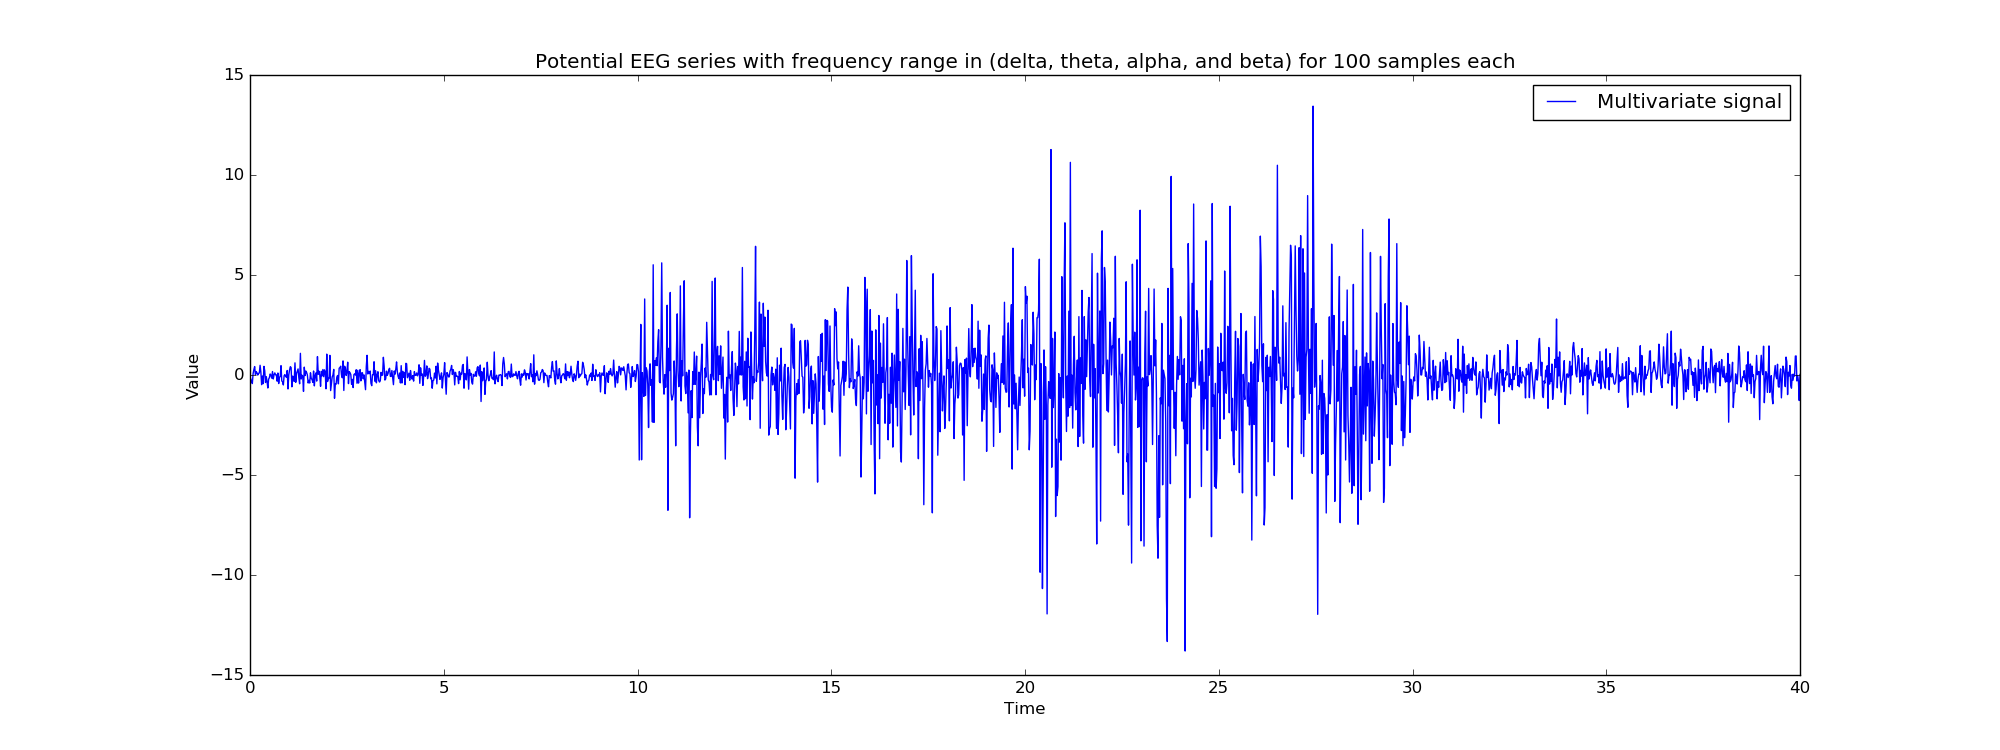
\includegraphics[width=1\textwidth]{images/changepoint_sd/ts}
  \caption{Time series formed by linear combination of sinusoidals with same frequency as that of brain signals.\label{fig:cp_sd_ts}}
\end{figure}

The peridogram is given by the function:
\begin{align}
  I_{k}(u) =& \frac{1}{2\pi n_{k}} {\lvert \sum_{j=\tau_{k-1}+1}^{\tau_{k}} Y_{j}e^{iju} \rvert}^{2}
\end{align}

The peridogram for this time series is given by:
\begin{figure}[ht!]
  \centering
  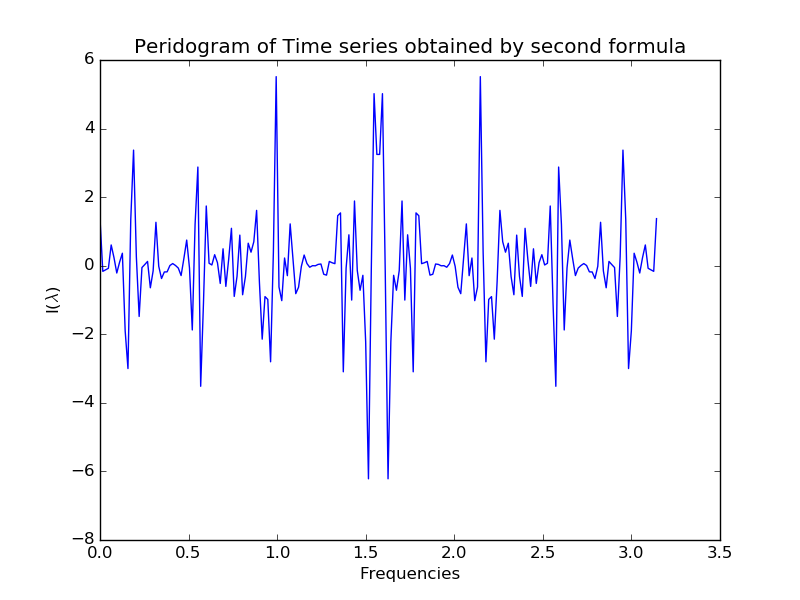
\includegraphics[width=1\textwidth]{images/changepoint_sd/peri2}
  \caption{Peridogram for the timeseries.\label{fig:cp_sd_peri2}}
\end{figure}

The energy of the window defined by $Y_{\tau_{k-1}+1}, \ldots, Y_{\tau_{k}}$ in frequency band $[\lambda_{j}, \mu_{j})$ is given by:
\begin{align}
  F_{kj} =& \int_{\lambda_{j}}^{\mu_{j}} I_{k}(u)du
\end{align}


The process for finding the energy band is still not clear.  In the below experiments we assume the energy band to lie between 0 and $\pi$.
The penality term is given by
\begin{align*}
  J_{n}(\tau, y) =& -\frac{1}{n} \sum_{k=1}^{k^{*}} (n_{k} \sum_{j=1}{J}F_{kj}^{2})
\end{align*}

The plot got by plotting J using a sliding window of 5s over the time series defined above is shown in figure below.
\begin{figure}[ht!]
  \centering
  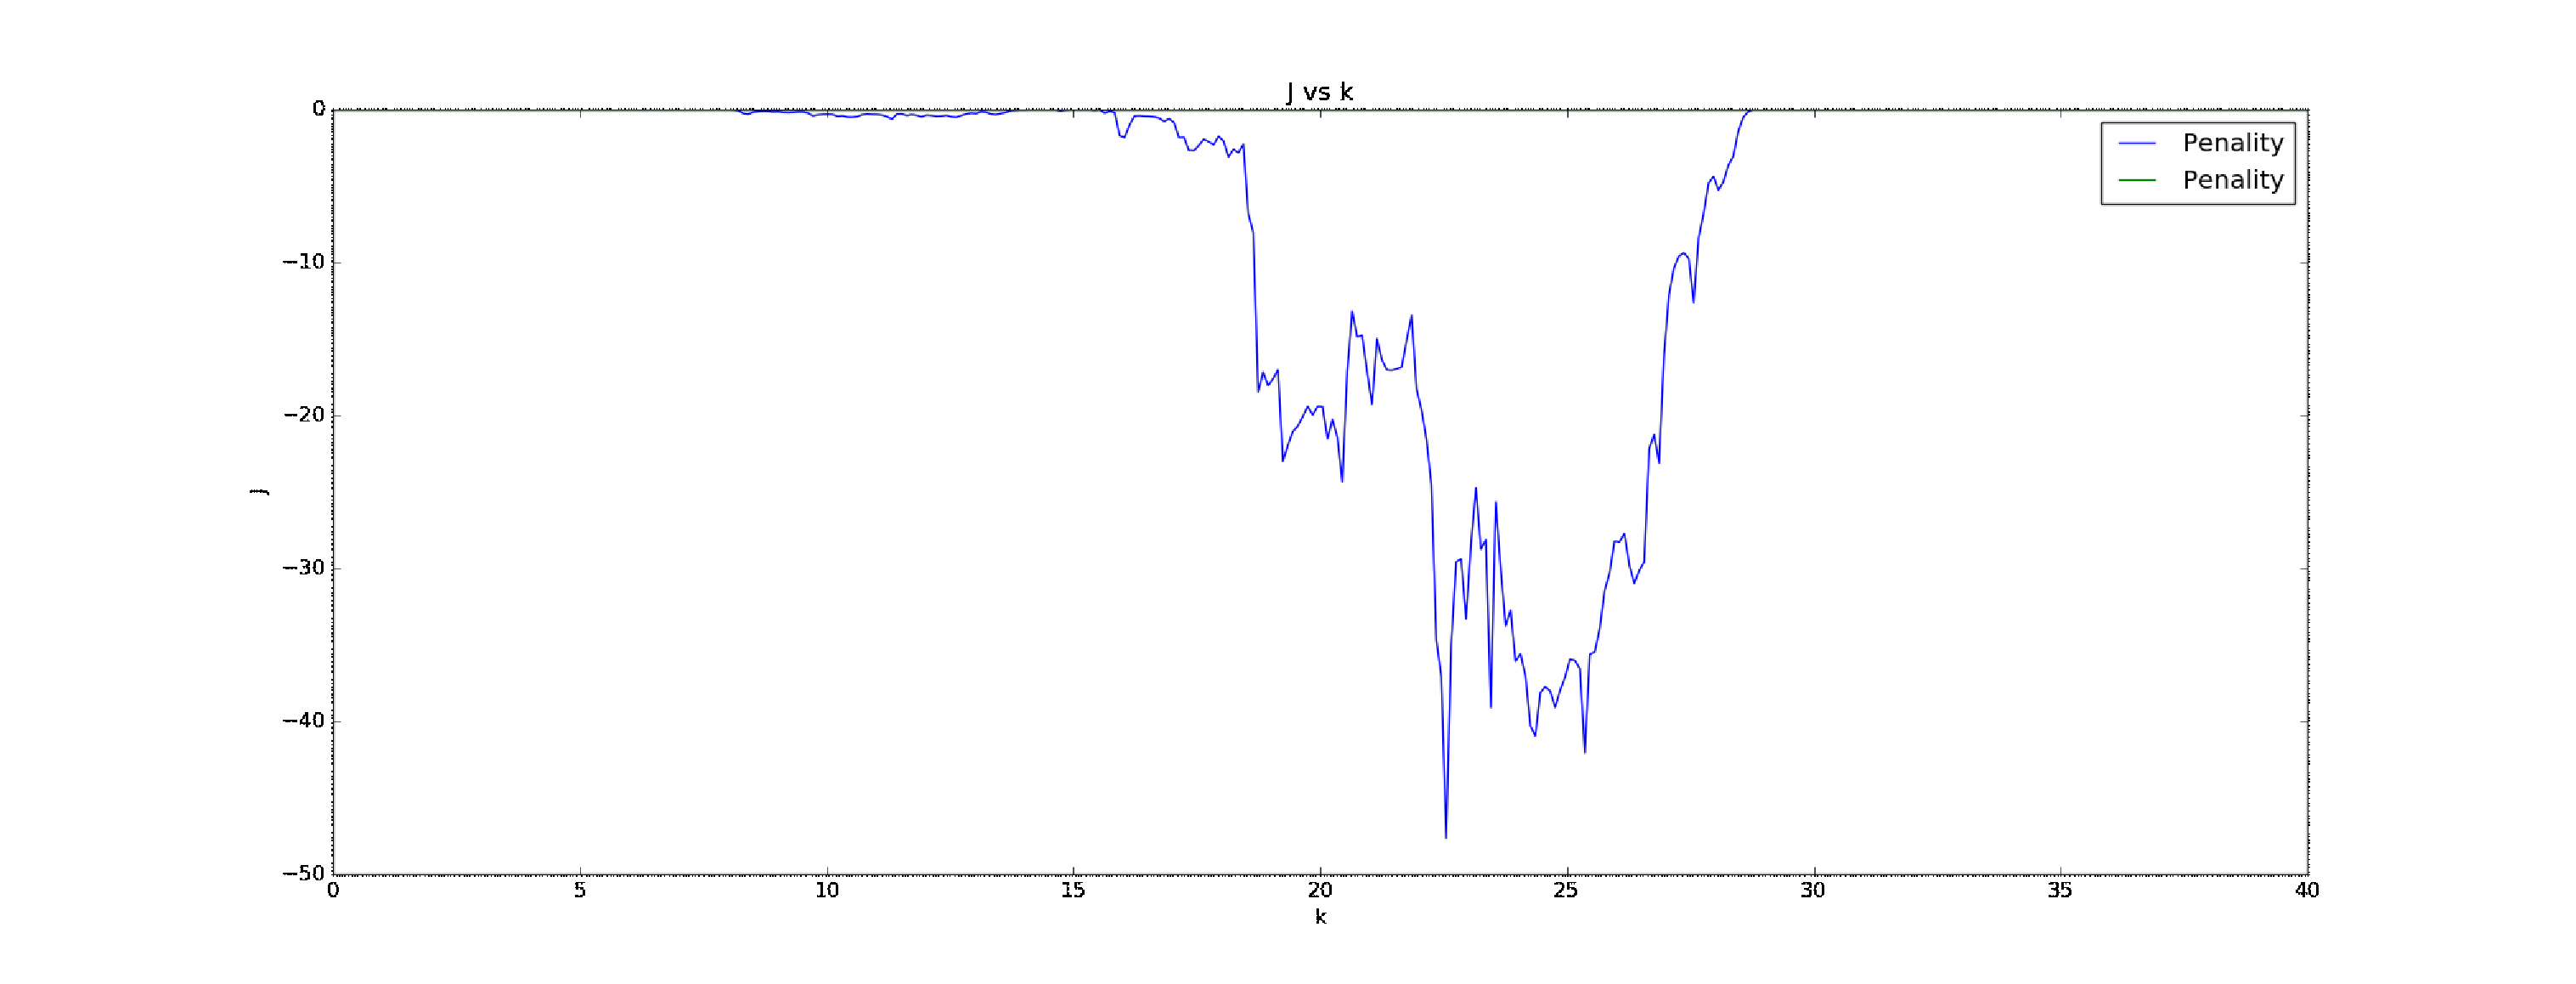
\includegraphics[width=1\textwidth]{images/changepoint_sd/penality}
  \caption{Penality vs k.\label{fig:cp_sd_penality}}
\end{figure}

\section{Questions}
\begin{itemize}
  \item The frequency range of a periodogram lies between $[0, \pi]$.  How to convert a frequency, say 12Hz, to the one viewable in periodogram 
  \item How to describe the energy landscape defined in equation 29 of~\cite{lavielle2005using}
\end{itemize}

\bibliographystyle{plain}
\bibliography{references}

\end{document}
